\documentclass{ctexart}
\usepackage{geometry}
\usepackage{fancyhdr}
\usepackage{graphicx}
\usepackage{booktabs}
\usepackage{amsmath}
\usepackage{diagbox}
\usepackage{tikz}
\usepackage{array}
\usepackage{zhnumber} % change section number to chinese
\renewcommand\thesection{\zhnum{section}}
\renewcommand \thesubsection {\arabic{subsection}}
\CTEXsetup[format={\Large\bfseries}]{section}

\geometry{
    a4paper,
    left=3.18cm,
    right=3.18cm,
    top=2.54cm,
    bottom=2.54cm
}

\pagestyle{fancy}
\fancyhf{}
\renewcommand{\headrulewidth}{0.7pt} % 设置页眉横线粗细
\fancyhead[L]{\kaishu\large 大学物理实验报告} % 在左侧设置页眉文字
\fancyhead[R]{\kaishu\large 哈尔滨工业大学(深圳) } % 在右侧设置页眉文字
\fancyfoot[R]{\raisebox{1\baselineskip}{\thepage}} % 将页数放在右下角


\setlength\headwidth{\textwidth}

\begin{document}

\noindent
\begin{center}
\textbf{
\begin{tabular}{p{2.4cm}p{2.4cm}p{4cm}p{4cm}}
    班级 \hrulefill & 学号 \hrulefill & 姓名 \hrulefill & 教师签字 \hrulefill \\
\end{tabular}
\begin{tabular}{p{6cm}p{3.6cm}p{3.6cm}}
    实验日期 \hrulefill & 预习成绩 \hrulefill & 总成绩 \hrulefill
\end{tabular}
{\noindent}	 \rule[-10pt]{\textwidth}{0.7pt}
}\end{center}

\begin{center}
    \Large \textbf{实验内容 \underline{RLC电路暂态特性的研究}}
\end{center}

\section{预习}
\subsection{RC、RL串联电路暂态过程电压表达式,以及时间常数$\tau$的表达式是什么?}
\subsection{RLC串联电路的暂态过程(三种阻尼过程)电压表达式、时间常数$\tau$表达式是什么?}
\subsection{请绘制数字示波器、信号发生器观测RC、RL和RLC串联电路的的连接线路示意图。}
\newpage
\section{原始数据记录}
\subsection{RC串联电路的暂态特性(使用方波信号进行实验,可取$V_{pp} = 10V$)}

$R= 500 \varOmega $方波信号周期$T=$ \rule{2cm}{0.5pt}

\begin{table}[htbp]
    \centering
    \begin{tabular}{|c|p{4em}|p{4em}|p{4em}|p{4em}|}
    \hline
    \diagbox[width=7em,height=1.7em]{$\tau$}{C} & \textbf{$0.022\mu F$} & \textbf{$10 \mu F$} & \textbf{$100\mu F$} & \textbf{$470\mu F$} \\
    \hline
    \textbf{时间常数$\tau$} & & & & \\
    \hline
    \end{tabular}
\end{table}

$C= 100 \mu F $方波信号周期$T=$ \rule{2cm}{0.5pt}

\begin{table}[htbp]
    \centering
    \begin{tabular}{|c|p{4em}|p{4em}|p{4em}|p{4em}|}
    \hline
    \diagbox[width=7em,height=1.7em]{$\tau$}{R} & \textbf{$10\Omega$} & \textbf{$50\Omega$} & \textbf{$100\Omega$} & \textbf{$500\Omega$} \\
    \hline
    \textbf{时间常数$\tau$} & & & & \\
    \hline
    \end{tabular}
\end{table}

\subsection{RL串联电路的暂态过程(使用方波信号进行实验,可取$V_{pp} = 10V$)}

$L= 10 mH $方波信号周期$T=$ \rule{2cm}{0.5pt}

\begin{table}[htbp]
    \centering
    \begin{tabular}{|c|p{4em}|p{4em}|p{4em}|}
    \hline
    \diagbox[width=7em,height=1.7em]{$\tau$}{R} & \textbf{$100\Omega$} & \textbf{$500\Omega$} & \textbf{$900\Omega$}  \\
    \hline
    \textbf{时间常数$\tau$} & & & \\
    \hline
    \end{tabular}
\end{table}

$R= 1000 \varOmega $方波信号周期$T=$ \rule{2cm}{0.5pt}

\begin{table}[!htbp]
    \centering
    \begin{tabular}{|c|p{4em}|p{4em}|p{4em}|}
    \hline
    \diagbox[width=7em,height=1.7em]{$\tau$}{L} & \textbf{$10mH$} & \textbf{$50mH$} & \textbf{$100mH$}  \\
    \hline
    \textbf{时间常数$\tau$} & & & \\
    \hline
    \end{tabular}
\end{table}

\subsection{RLC串联电路的暂态特性(使用方波信号进行实验,可取$V_{pp} = 10V$)}

\begin{center}
    测量欠阻尼情况下$U_C$充电时振荡波形的任一$t1$时峰值$U_{ct_1 }$和t1+nT时峰值$U_{c(t_1+nT)}$
\end{center}

$R = $\rule{2cm}{0.5pt},  $C = $\rule{2cm}{0.5pt}, $L = $\rule{2cm}{0.5pt}

方波信号周期$T = $\rule{2cm}{0.5pt}

\begin{table}[!htbp]
    \centering
    \begin{tabular}{|c|p{2em}|p{2em}|p{2em}|p{2em}|p{2em}|p{2em}|p{2em}|p{2em}|p{2em}|}
    \hline
    $n$ & 0 & 1 & 2 & 3 & 4 & 5 & 6 & 7 & 8 \\
    \hline
    $Uc(t1+nT)$ & & & & & & & & & \\
    \hline
    \end{tabular}
\end{table}

$E = $\rule{2cm}{0.5pt},  $t_1 = $\rule{2cm}{0.5pt}

\begin{tikzpicture}[remember picture,overlay]
    \node[anchor=south east,inner sep=100pt] at (current page.south east) {
        \renewcommand{\arraystretch}{1.5} % 表格行高倍数
        \setlength{\tabcolsep}{18pt}    
    \begin{tabular}{|c|c|}
        \hline
        \LARGE  教师 & \LARGE  姓名 \\
        \hline
        \LARGE \kaishu 签字 &  \\
        \hline
        \end{tabular}
    };
\end{tikzpicture}
\newpage

\section{数据处理}

\subsection{记录各项实验任务过程中的R、C和L各参数值,示波器观察到的波形,以及时间常数$\tau$。}

在实验中,RC与RL电路中均出现了良好的预期图像,即如同所示曲线:

RC,LC曲线均与下图相似:
\begin{figure}[h]
    \centering
    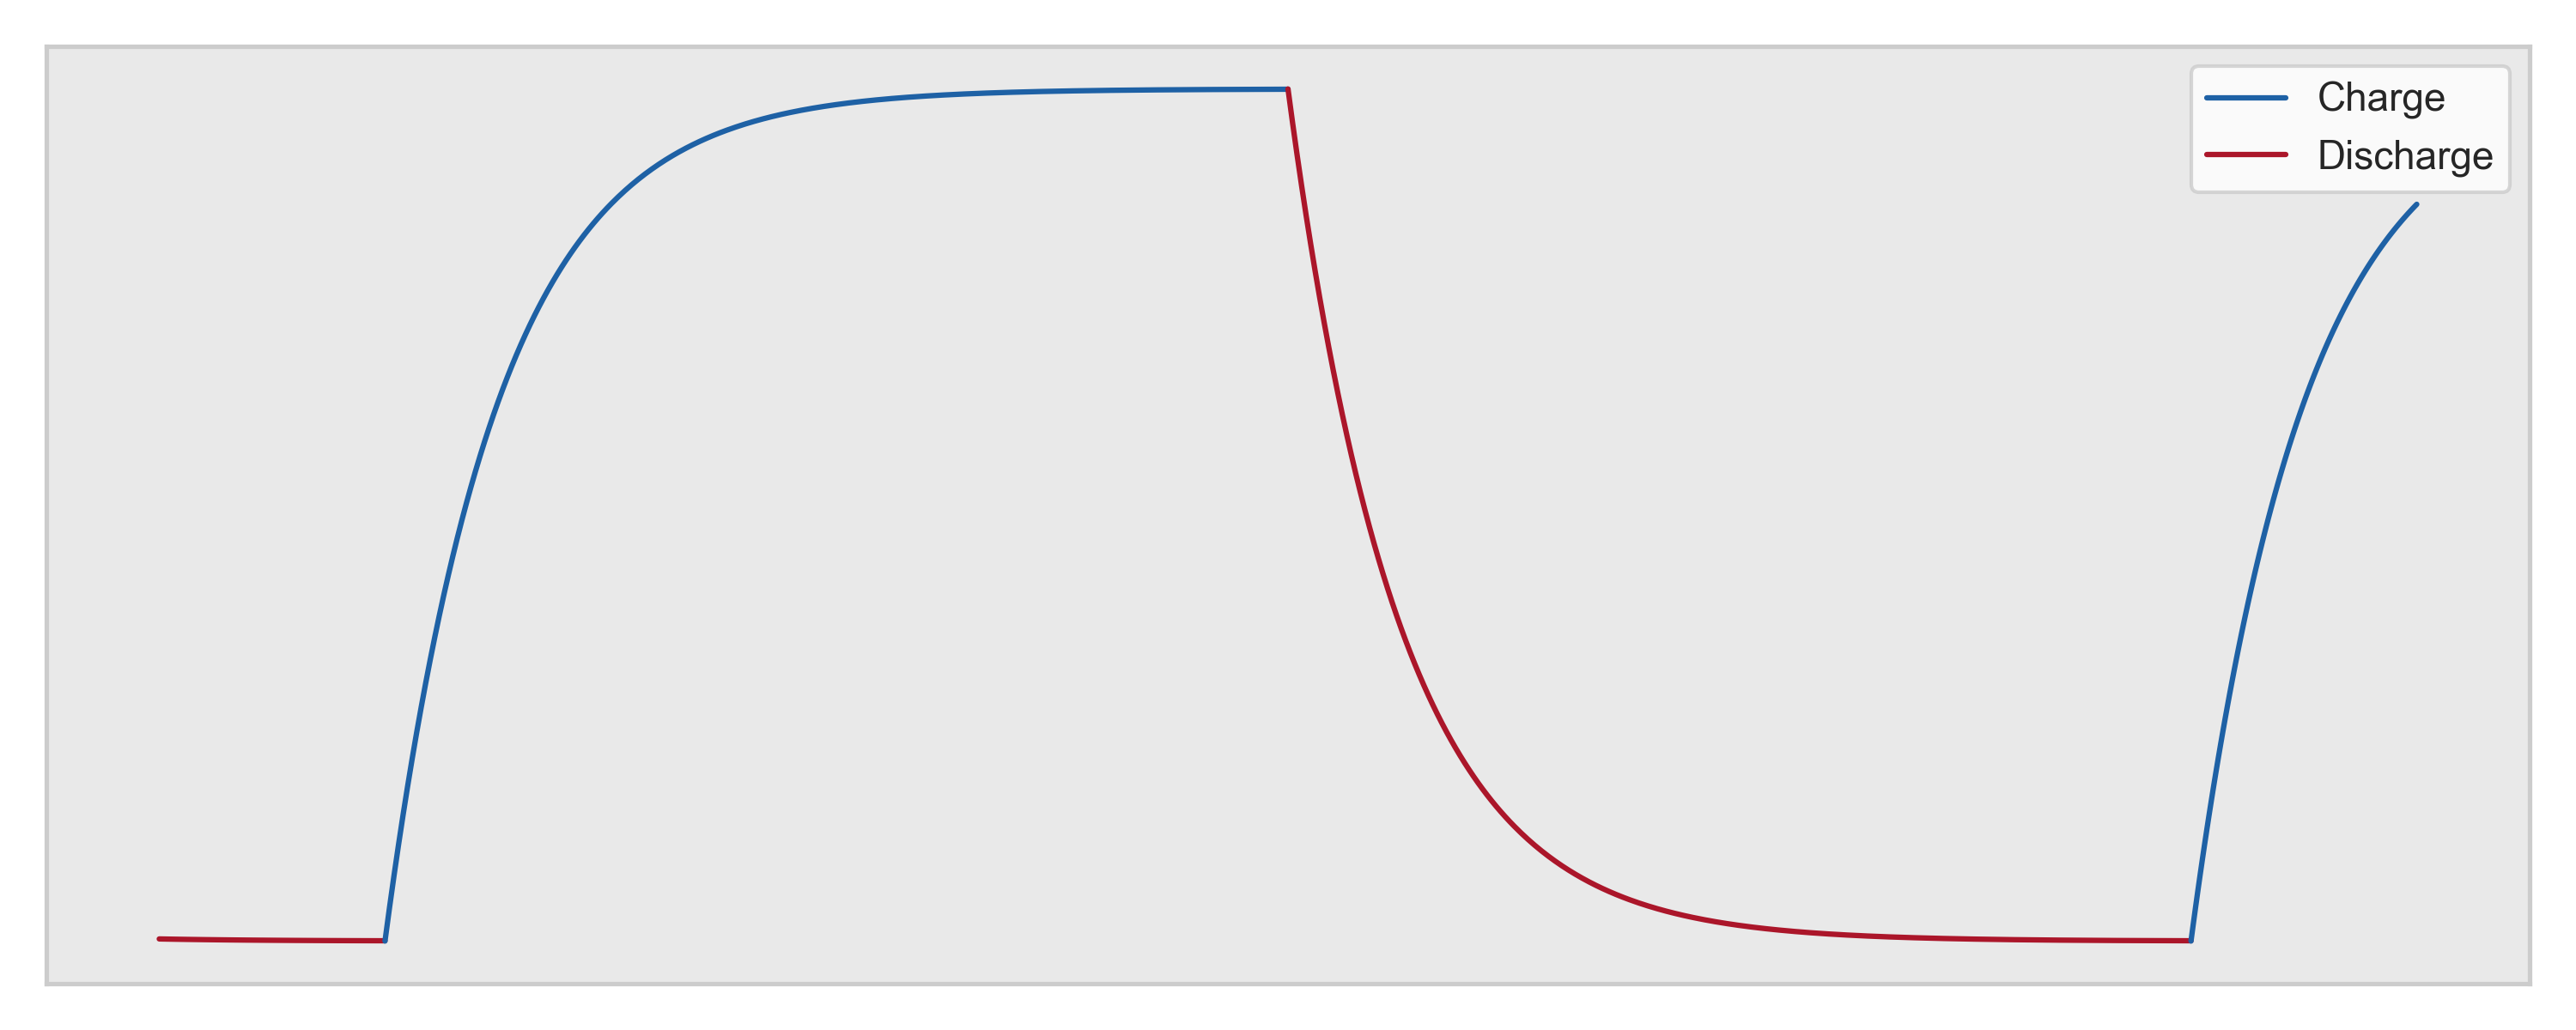
\includegraphics[width=.9\textwidth]{pic.png} % 插入左侧图像
    \caption{RC,LC曲线}
    \label{fig: rclc-pic}
\end{figure}

RLC的欠阻尼情况与下图相似:

\begin{figure}[h]
    \centering
    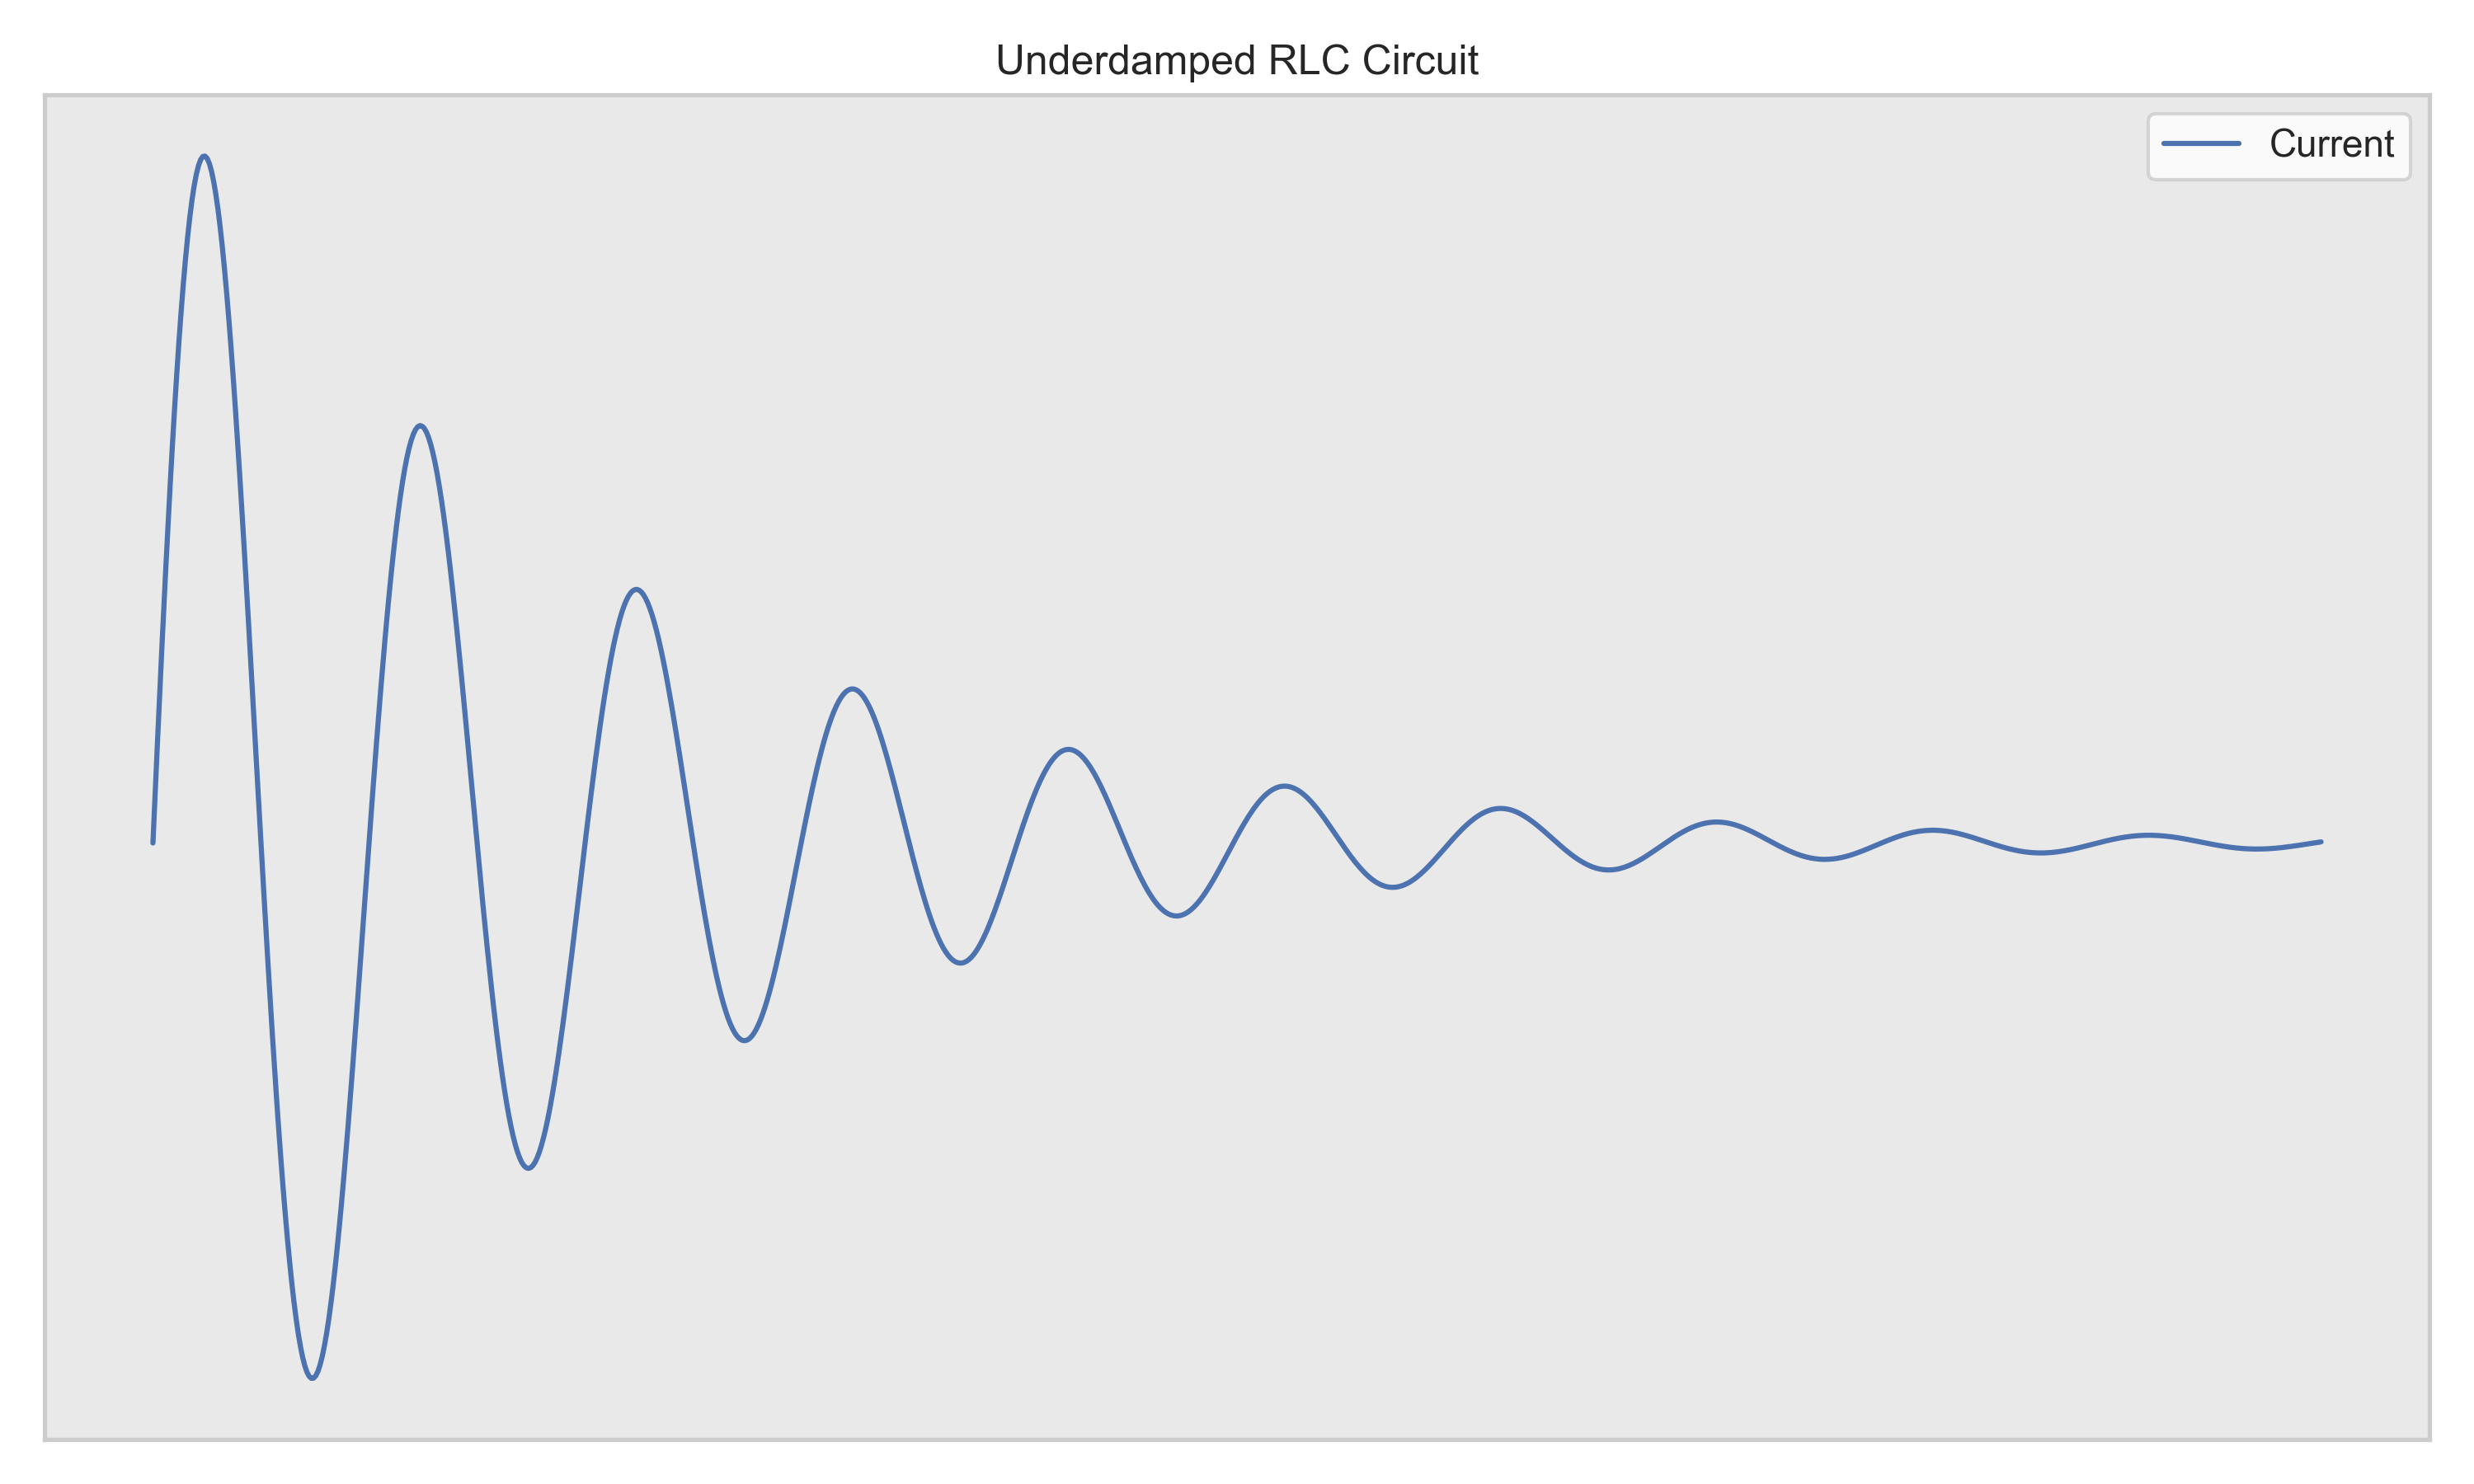
\includegraphics[width=.9\textwidth]{pic-rlc.png} % 插入左侧图像
    \caption{RLC曲线}
    \label{fig: rlc-pic}
\end{figure}

理论推演结果与实际结果符合,故认为实验较为理想,相关数据记录在上页

\subsection{测量欠阻尼情况下$U_C$充电时振荡波形的任一$t_1$时峰值$U_{ct_1}$和$t_1+nT$时峰值$U_{c(t_1+nT)}$,采用最小二乘法或作图法求出$ \ln\left(\frac{U_C}{E}-1\right) \sim t$的斜率,计算时间常数$\tau$,并与理论值 $\tau = \frac{2L}{R}$($R=R_\text{\songti 阻}+ R_S+ R_L$)进行比较,分析误差产生的原因}

理论显示波峰出现的周期$T$应为定值,故在实验中采取逐差法,记得$T = 94.2 \mu s$,通过调用numpy库计算$\ln\left(\frac{U_C}{E}-1\right)$的值,如下表所示:

\begin{table}[h]
    \centering
    \caption{$ \ln\left(\frac{U_C}{E}-1\right) \sim t$}
    \label{tab:Ks}
    \begin{tabular}{ c | c c c c c c c c c}
      \toprule
      $t(\mu s)$  & 48.0 & 142.2 & 236.4 & 330.6 & 424.8 & 519.0 & 613.2 & 707.4 & 801.6 \\
      \hline
      $\ln\left(\frac{U_C}{E}-1\right)$ & -0.22 & -0.71 & -1.14 & -1.61 & -2.12 & -2.81 & -3.22 &  -3.50 & -4.60 \\
      \bottomrule
    \end{tabular}
\end{table}

利用最小二乘法进行计算,在python中矩阵计算较为方便,所以使用与教材所给公式等价的方式进行计算:

$$ 
A = {\begin{bmatrix}
    1 & 1 & \cdots & 1 \\
    48.0 & 142.2 & \cdots & 801.6 
 \end{bmatrix}}^T \ \ \ \
  Y = {\begin{bmatrix} -0.22  & -0.71 & \cdots & -4.60 \end{bmatrix}}^T
$$

带入公式:
$$ 
\widehat{K} = {(A^T A)}^{-1} A^T Y 
$$

其中$ \widehat{K} = {\begin{bmatrix} k_0  & k_1 & \cdots & k_{n-1} & k_{n} \end{bmatrix}}^T $ 即为所求。

~

计算得:
$$\widehat{K} = \begin{bmatrix}   -0.134 \\ -0.00552 \end{bmatrix} $$

即经过最小二乘回归得到$\frac{1}{\tau} = 0.00552 $(t单位为$\mu s$时),实际运算得到数据$\frac{1}{\tau} = \frac{R}{2L} = 5000$,这里的$5000$是对于$s$的,故对于$\mu s$则为$0.005$,实验间接得到的数据相对于理论值偏小,经分析有以下可能:

\begin{itemize}
    \item $\frac{1}{\tau}$的理论计算式中,$R$位于分母上,而计算时仅仅套用了电阻的阻值,实际上其他电子元件也存在一定阻值,于是使得间接测量值偏大一些,这应当是实验误差的主要来源。
    \item 其次,物理模型假设为理想条件下进行的运算,而实际情况可能会有相对复杂的模型结构。
    \item 同时在测量中也存在随机误差,在测量电路中的电压,电流等物理量时,仪器的精度,灵敏度以及测量方法的精确性都会影响实验结果。
    \item 同时实验环境可能存在电磁干扰,温度变化等额外因素,这些因素对需要精确测量的物理量可能会造成影响。
\end{itemize}

\newpage

\section{实验现象分析及结论}
\subsection{RC电路}

\begin{itemize}
    \item 在RC电路中,当施加一个方波或者一个充电电压时,电容会充电或者放电。初始时,电容会迅速充电或放电,随后充电/放电速度逐渐减缓,直至达到稳态。当施加方波信号时,电压响应呈现出充电/放电过程中的典型指数衰减或增长。
    \item 这种现象可以通过RC电路的特性来解释。电容会阻碍电流的变化,因此在开始时,电容允许电流快速通过,然后随着时间的推移,电容会充电或放电,电流减小,直到最终达到稳态。指数衰减的特性是RC电路响应的一个重要特征,其时间常数$\tau = RC$ 决定了充电/放电过程的速度。
\end{itemize}

\subsection{RL电路}

\begin{itemize}
    \item 在RL电路中,当施加一个方波或者一个电压脉冲时,电感会产生反向电动势,导致电感电流增加。初始时,电感电流增加迅速,然后逐渐达到稳态。
    \item 这种现象可以通过RL电路的特性来解释。电感会阻碍电流的变化,初始时,电感中没有电流,施加电压时,电感会产生反向电动势,试图阻止电流的变化,从而导致电流增加。随着时间的推移,电感电流逐渐增加,直到达到稳态。
\end{itemize}

\subsection{RLC电路}

\begin{itemize}
    \item 在RLC电路中,当施加一个方波或者一个电压脉冲时,电路中会出现振荡现象。振荡的频率和振幅取决于电路的参数和驱动信号。对于不同的电子原件出现了大致三类曲线。
    \item 振荡的发生是由于电容和电感之间的能量交换。当施加激励时,电容开始充电或放电,而电感则试图保持电流不变。这种电荷和电流的变化导致了电路中的能量在电容和电感之间的周期性转换,从而产生振荡。振荡的频率取决于电感、电容和电阻的数值,以及激励信号的特性。
\end{itemize}

\section{讨论题}

\subsection{在RC和RL电路中,固定方波频率$f$而改变R的阻值,为什么会有各种不同的波形?若固定R而改变方波频$f$,会得到类似的波形吗?为什么?}

在RC电路中,当R足够小时,充放电时间变短,两个相邻的充放电曲线中间电压保持水平时间相对于充放电的时间要变长;而R足够大时,波形会逐渐变成三角波的形状,这是因为电容器还没有来得及充满电,两级电压就发生了反转,导致电容器开始放电。

在RL电路中,$\tau$中$R$的计算位置变化,于是会形成与RC电路相反的结果,R足够小,逐渐形成三角波,R足够大,两个相邻的充放能曲线中间电压保持水平时间相对于充放能的时间要变长。

在两种电路中,若固定R而改变方波频 $f$,单独充放电(充能放能)过程关于时间的函数是不变的,但是$f$的改变会改变充放电(充能放能)的时间,如果$f$变小,则电路有了更多的时间进行充放电(充能放能),两个充放电(充能放能)曲线之间的间隔会被拉长;而如果$f$变大,那么信号发生器就不会给电路足够的时间进行充放电(充能放能),逐渐形成三角波。

\subsection{在RLC电路中,为什么要适当调节方波频率才能观测到阻尼振荡的波形?如果频率很高,将会发生什么样的情况?试观察。}


如果方波信号的频率过高,电路还没有形成稳定的状态就会进行下一步响应,导致本应当形成的曲线被扰乱,无法实现实验效果。

当频率过低时,由于低频信号引起的充放电过程较为缓慢,可能需要较长的时间才能使电路达到稳定状态。因此,在低频情况下,观察到的响应可能需要更长的时间才能显现出来。

\end{document}